\section{Methodik}

In diesem Kapitel wird der in dieser Arbeit verfolgte methodische Ansatz zur 
semi-supervisierten Videoannotation beschrieben. Ziel ist es, den manuellen 
Annotierungsaufwand bei video-basierten Luftaufnahmen deutlich zu reduzieren, 
ohne dabei die Qualität der erzeugten Annotationen wesentlich zu beeinträchtigen. 
Hierzu wird ein iterativer Ansatz vorgestellt, der Transfer Learning, 
Objektverfolgung und Pseudo-Labeling miteinander kombiniert.

Der zentrale Gedanke des Ansatzes besteht darin, lediglich eine kleine Teilmenge 
der Videoframes manuell zu annotieren und diese als Ausgangspunkt für das Training 
eines vortrainierten Objekterkennungsmodells zu nutzen. Auf Basis dieses Modells 
werden anschließend nicht annotierte Zwischenframes automatisch analysiert. Die 
dabei erzeugten Detektionen werden mithilfe eines Tracking-Verfahrens zeitlich 
verknüpft, um konsistente Objekttrajektorien über mehrere Frames hinweg zu 
erhalten.

Die aus der Objektverfolgung resultierenden Informationen werden genutzt, um 
automatisch zusätzliche Annotationen in Form von sogenannten Pseudo-Labels zu 
erzeugen. Durch den Einsatz einfacher heuristischer Kriterien, wie 
Konfidenzschwellwerten und minimalen Tracking-Dauern, wird die Qualität dieser 
Pseudo-Labels kontrolliert. Die so erweiterten Annotationen dienen anschließend 
als Trainingsdaten für eine erneute Modellanpassung im Sinne eines iterativen 
Self-Training-Prozesses.

Der beschriebene Ansatz ist modular aufgebaut und erlaubt es, einzelne 
Komponenten wie die Anzahl der Iterationen, die Tracking-Strategie oder die 
Filterkriterien flexibel anzupassen. Dadurch eignet sich der vorgestellte 
Ansatz insbesondere für reale Anwendungsszenarien mit begrenzten manuellen 
Annotierungsressourcen und großen Mengen an Videodaten.


\newpage

\usetikzlibrary{shapes.geometric, arrows.meta, positioning, calc}

\begin{figure}[htbp]
    \centering
    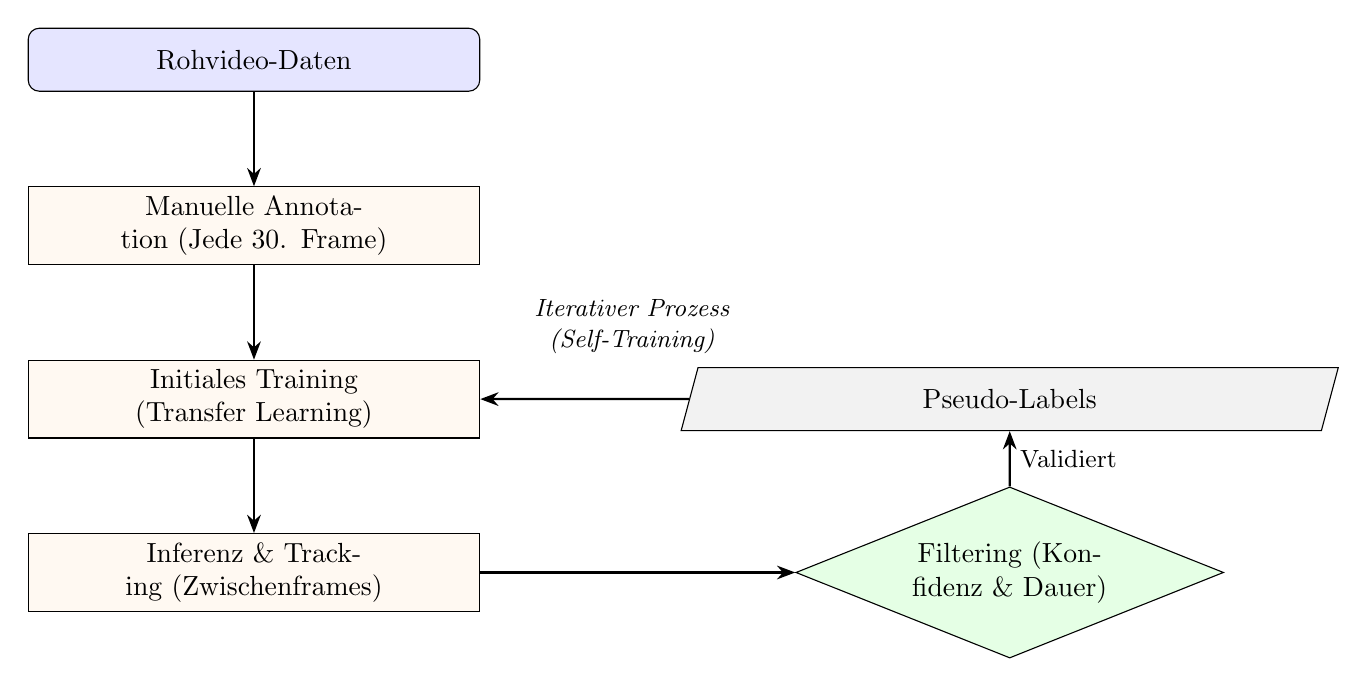
\begin{tikzpicture}[
        % Yatay mesafeyi (4.5cm) ve dikey mesafeyi (1.2cm) ayarladık
        node distance=1.2cm and 4cm,
        auto,
        % Kutuların genişliğini tek satıra sığacak şekilde 5.5cm yaptık
        startstop/.style={rectangle, rounded corners, draw, fill=blue!10, text width=5.5cm, align=center, minimum height=0.8cm},
        process/.style={rectangle, draw, fill=orange!5, text width=5.5cm, align=center, minimum height=0.8cm},
        decision/.style={diamond, draw, fill=green!10, text width=3.5cm, align=center, inner sep=0pt, aspect=2.5},
        data/.style={trapezium, draw, fill=gray!10, trapezium left angle=75, trapezium right angle=105, text width=4.5cm, align=center, minimum height=0.8cm},
        arrow/.style={-Stealth, thick}
    ]

    % Düğümler (Nodes) - Metinler artık tek satır
    \node (start) [startstop] {Rohvideo-Daten};
    
    \node (manual) [process, below=of start] {Manuelle Annotation (Jede 30. Frame)};
    
    \node (train) [process, below=of manual] {Initiales Training (Transfer Learning)};
    
    \node (inference) [process, below=of train] {Inferenz \& Tracking (Zwischenframes)};
    
    % Sağ taraf
    \node (filter) [decision, right=of inference] {Filtering (Konfidenz \& Dauer)};
    
    \node (pseudo) [data] at (train -| filter) {Pseudo-Labels};

    % Oklar (Arrows)
    \draw [arrow] (start) -- (manual);
    \draw [arrow] (manual) -- (train);
    \draw [arrow] (train) -- (inference);
    \draw [arrow] (inference) -- (filter);
    \draw [arrow] (filter) -- node[right, font=\small] {Validiert} (pseudo);
    \draw [arrow] (pseudo) -- (train);

    % Döngü Etiketi
    \node [font=\small\itshape, text width=4cm, align=center, anchor=south] 
        at ($(pseudo.north)!0.5!(train.north)$) {Iterativer Prozess (Self-Training)};

    \end{tikzpicture}
    \caption{Methodischer Ablauf: Iterative Video-Annotation mittels Transfer Learning, Tracking und Pseudo-Labeling.}
    \label{fig:methodik_workflow}
\end{figure}

\subsection{Gesamtübersicht des Ansatzes}

Der in dieser Arbeit verfolgte Ansatz zielt darauf ab, den manuellen Aufwand für die 
Annotation video-basierter Luftaufnahmen deutlich zu reduzieren. Hierzu wird ein 
semi-supervisiertes Verfahren eingesetzt, das Transfer Learning, Objektverfolgung 
sowie automatische Label-Propagation kombiniert. Der Ansatz ist insbesondere für 
Szenarien geeignet, in denen große Mengen an Videodaten vorliegen, eine vollständige 
manuelle Annotation jedoch nicht praktikabel ist.

Ausgangspunkt des Verfahrens ist eine begrenzte Menge manuell annotierter Videoframes, 
die in regelmäßigen Abständen aus den Rohvideos extrahiert werden. Diese sparsam 
annotierten Frames dienen als Trainingsgrundlage für ein vortrainiertes 
Objekterkennungsmodell. Das Modell wird nicht von Grund auf neu trainiert, sondern im 
Sinne des Transfer Learnings an die domänenspezifischen Inhalte der Luftaufnahmen 
angepasst.

Das initial trainierte Modell wird anschließend auf nicht annotierte Zwischenframes 
angewendet, um potenzielle Objekte automatisch zu detektieren. Da es sich um 
Videodaten handelt, weisen die Detektionen eine zeitliche Abhängigkeit zwischen 
aufeinanderfolgenden Frames auf. Um diese zeitliche Konsistenz gezielt auszunutzen, 
wird ein Objektverfolgungsverfahren eingesetzt, das Detektionen über mehrere Frames 
hinweg miteinander verknüpft und stabile Objekttrajektorien erzeugt.

Auf Basis der verfolgten Objekttrajektorien werden zusätzliche Annotationen in Form 
von sogenannten Pseudo-Labels generiert. Um die Qualität dieser automatisch erzeugten 
Labels sicherzustellen, kommen einfache heuristische Filter zum Einsatz, etwa 
Schwellwerte für Detektionskonfidenzen oder Mindestdauern von Objekttracks. Die so 
gewonnenen Pseudo-Labels erweitern den ursprünglichen Trainingsdatensatz.

Dieser erweiterte Datensatz kann anschließend für eine erneute Modellanpassung 
verwendet werden. Durch eine optionale iterative Wiederholung dieses Prozesses wird 
ein Self-Training-Ansatz realisiert, der es erlaubt, die Leistungsfähigkeit des 
Objekterkennungsmodells schrittweise zu verbessern, ohne den manuellen 
Annotierungsaufwand signifikant zu erhöhen. Die einzelnen Komponenten des Ansatzes 
sind modular aufgebaut und können abhängig von den experimentellen Ergebnissen 
angepasst oder vereinfacht werden.


\begin{figure}[htbp]
    \centering
    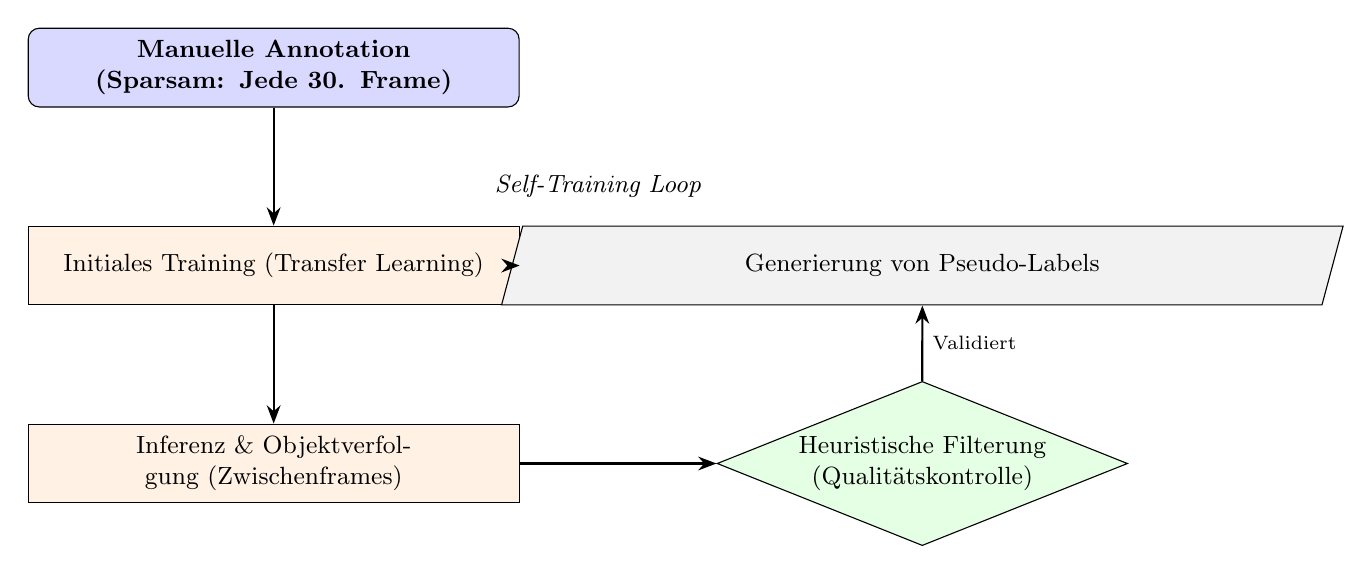
\begin{tikzpicture}[
        node distance=1.5cm and 2.5cm,
        auto,
        manual_style/.style={rectangle, rounded corners, draw, fill=blue!15, text width=6cm, align=center, minimum height=1cm, font=\small\bfseries},
        auto_style/.style={rectangle, draw, fill=orange!10, text width=6cm, align=center, minimum height=1cm, font=\small},
        decision_style/.style={diamond, draw, fill=green!10, text width=3.5cm, align=center, inner sep=0pt, aspect=2.5, font=\small},
        data_style/.style={trapezium, draw, fill=gray!10, trapezium left angle=75, trapezium right angle=105, text width=5cm, align=center, minimum height=1cm, font=\small},
        line/.style={-Stealth, thick}
    ]

    % Dikey Ana Akış (Manual -> Initial Training)
    \node (manual) [manual_style] {Manuelle Annotation (Sparsam: Jede 30. Frame)};
    \node (train) [auto_style, below=of manual] {Initiales Training (Transfer Learning)};
    \node (inference) [auto_style, below=of train] {Inferenz \& Objektverfolgung (Zwischenframes)};

    % Sağ Taraf (Iteratif Döngü)
    \node (filter) [decision_style, right=of inference] {Heuristische Filterung \\ (Qualitätskontrolle)};
    \node (pseudo) [data_style] at (train -| filter) {Generierung von Pseudo-Labels};

    % Bağlantılar
    \draw [line] (manual) -- (train);
    \draw [line] (train) -- (inference);
    \draw [line] (inference) -- (filter);
    \draw [line] (filter) -- node[right, font=\scriptsize] {Validiert} (pseudo);
    \draw [line] (pseudo) -- (train);

    % Döngü Açıklaması
    \node [font=\small\itshape, text width=4cm, align=center] at ($(pseudo.north)!0.5!(train.north) + (0,0.5)$) {Self-Training Loop};

    \end{tikzpicture}
    \caption{Gesamtübersicht des semi-supervisierten Ansatzes zur iterativen Videoannotation.}
    \label{fig:methodik_overall}
\end{figure}

\subsection{Basismodell und Transfer Learning}

Als Basismodell wird in dieser Arbeit ein YOLO-basiertes Objekterkennungsmodell 
verwendet, das für allgemeine Objekterkennungsaufgaben vortrainiert wurde. Modelle 
der YOLO-Familie zeichnen sich durch ihren einstufigen Aufbau aus, bei dem 
Objektlokalisierung und Klassifikation in einem gemeinsamen Vorwärtsschritt 
durchgeführt werden. Dadurch eignen sie sich besonders für video-basierte 
Anwendungsszenarien, in denen sowohl eine hohe Detektionsgenauigkeit als auch eine 
effiziente Inferenz erforderlich sind.

Das Training des Modells erfolgt nicht von Grund auf neu. Stattdessen werden die 
vortrainierten Modellgewichte als Ausgangspunkt genutzt und im Rahmen des Transfer 
Learnings an die domänenspezifischen Eigenschaften der verwendeten Luftaufnahmen 
angepasst. Diese Entscheidung basiert auf der Beobachtung, dass insbesondere bei 
begrenzter Verfügbarkeit manuell annotierter Trainingsdaten ein Training mit 
zufälliger Initialisierung zu instabilen Lernverläufen und einer erhöhten 
Überanpassung führen kann. Durch die Nutzung vortrainierter Gewichte können bereits 
gelernte allgemeine visuelle Merkmale, wie Kanten, Texturen und einfache Formen, 
direkt übernommen werden.

Im Rahmen des Transfer-Learning-Prozesses werden die vorhandenen Modellgewichte als 
Initialisierung verwendet, während die Ausgabeschichten an die im Ziel-Datensatz 
definierten Objektklassen angepasst werden. Das Modell wird anschließend mithilfe 
der sparsam annotierten Videoframes feinjustiert. Dabei liegt der Fokus nicht auf 
einer vollständigen Neuanpassung aller Merkmale, sondern auf der schrittweisen 
Anpassung höherer Repräsentationsebenen an die spezifischen visuellen Eigenschaften 
von UAV-Aufnahmen, wie veränderte Perspektiven, geringe Objektgrößen und komplexe 
Hintergrundstrukturen.

Durch dieses Vorgehen wird erreicht, dass das Modell bereits in frühen 
Trainingsphasen sinnvolle Detektionen erzeugen kann, obwohl nur eine begrenzte 
Anzahl manuell annotierter Beispiele zur Verfügung steht. Diese Eigenschaft ist 
insbesondere für den weiteren Verlauf des vorgeschlagenen Ansatzes von Bedeutung, 
da das initial trainierte Modell als Grundlage für die automatische Annotation 
nicht beschrifteter Zwischenframes dient.

Zusammenfassend stellt das eingesetzte Transfer-Learning-Verfahren einen zentralen 
Baustein des gesamten Ansatzes dar. Es ermöglicht eine stabile Initialisierung des 
Objekterkennungsmodells, reduziert den Bedarf an umfangreichen manuellen 
Annotationen und schafft die Voraussetzung für die nachgelagerten Schritte der 
Objektverfolgung, Pseudo-Label-Generierung und iterativen Modellanpassung.

\subsection{Automatische Annotation durch Pseudo-Labeling}

Im nächsten Schritt des vorgeschlagenen Ansatzes wird das initial mittels Transfer 
Learning trainierte Objekterkennungsmodell eingesetzt, um nicht manuell annotierte 
Zwischenframes automatisch zu analysieren. Die dabei erzeugten Detektionen werden 
als sogenannte Pseudo-Labels interpretiert und bilden die Grundlage für eine 
schrittweise Erweiterung des Trainingsdatensatzes.

Ziel des Pseudo-Labeling-Verfahrens ist es, ausgehend von einer begrenzten Anzahl 
manuell annotierter Frames eine deutlich größere Menge an Trainingsdaten zu 
generieren. Auf diese Weise soll die Generalisierungsfähigkeit des Modells verbessert 
werden, ohne den manuellen Annotierungsaufwand proportional zur Datenmenge zu erhöhen. 
Die vom Modell erzeugten Vorhersagen werden jedoch nicht ungefiltert übernommen, 
sondern einer gezielten Qualitätskontrolle unterzogen.

Um die Zuverlässigkeit der automatisch erzeugten Annotationen sicherzustellen, 
werden Pseudo-Labels nur dann akzeptiert, wenn sie vordefinierte heuristische 
Kriterien erfüllen. Dazu zählen insbesondere Mindestschwellwerte für die 
Detektionskonfidenz sowie die zeitliche Konsistenz der Detektionen über mehrere 
aufeinanderfolgende Videoframes hinweg. Diese Filtermechanismen reduzieren die 
Wahrscheinlichkeit, dass vereinzelte Fehlklassifikationen oder instabile Detektionen 
in den Trainingsprozess eingehen.

Ein wesentlicher Vorteil der hier betrachteten Videoaufnahmen liegt in ihrer 
zeitlichen Struktur. Durch die Nutzung eines Objektverfolgungsverfahrens können 
Detektionen desselben Objekts über mehrere Frames hinweg miteinander verknüpft werden. 
Die daraus resultierenden Objekttrajektorien ermöglichen es, Pseudo-Labels nicht nur 
frameweise, sondern auf Basis konsistenter zeitlicher Zusammenhänge zu erzeugen. 
Dadurch wird die Robustheit der automatischen Annotation zusätzlich erhöht.

Die auf diese Weise generierten Pseudo-Labels werden mit den ursprünglich manuell 
annotierten Daten zusammengeführt und bilden einen erweiterten Trainingsdatensatz. 
Dieser Datensatz dient als Grundlage für eine erneute Anpassung des 
Objekterkennungsmodells. Durch eine optionale iterative Wiederholung dieses Prozesses 
kann ein Self-Training-Mechanismus realisiert werden, bei dem sich die Modellleistung 
schrittweise verbessert.

Das Pseudo-Labeling stellt somit einen zentralen Bestandteil des vorgestellten 
semi-supervisierten Ansatzes dar. Gleichzeitig ist die Qualität der erzeugten Labels 
stark von der Leistungsfähigkeit des initialen Modells sowie von den gewählten 
Filterstrategien abhängig. Eine sorgfältige Auswahl dieser Parameter ist daher 
entscheidend für die Stabilität und Zuverlässigkeit des gesamten 
Anotationsprozesses.

\subsection{Objektverfolgung zur Label-Propagation}

Ein zentraler Bestandteil des vorgeschlagenen semi-supervisierten 
Anotationsansatzes ist der gezielte Einsatz von Objektverfolgung zur aktiven 
Unterstützung der Label-Propagation. Im Gegensatz zu rein framebasierten 
Verfahren wird die zeitliche Kontinuität von Objekten in Videosequenzen explizit 
ausgenutzt, um automatisch erzeugte Annotationen robuster und konsistenter zu 
gestalten.

Die Objektverfolgung baut in dieser Arbeit auf den Ausgaben des zuvor trainierten 
Objekterkennungsmodells auf. Detektionen in aufeinanderfolgenden Videoframes werden 
anhand räumlicher Überlappung, zeitlicher Nähe sowie optionaler 
Erscheinungsmerkmale miteinander verknüpft. Auf diese Weise entstehen 
Objekttrajektorien, die es erlauben, einzelne Detektionen als zusammengehörige 
Beobachtungen desselben Objekts über die Zeit zu interpretieren.

Die aus der Objektverfolgung gewonnenen zeitlichen Informationen werden gezielt 
für die Generierung zusätzlicher Pseudo-Labels genutzt. Ein Objekttrack, der über 
eine Mindestanzahl aufeinanderfolgender Frames stabil verfolgt werden kann, dient 
als Indikator für die Zuverlässigkeit der zugrunde liegenden Detektionen. 
Kurzlebige oder inkonsistente Detektionen werden dadurch effektiv aus dem 
Pseudo-Labeling-Prozess ausgeschlossen.

Darüber hinaus ermöglicht die Objektverfolgung die gezielte Übertragung von 
Annotationen zwischen benachbarten Frames. Klassen- und Positionsinformationen 
von manuell annotierten Objekten können entlang eines konsistenten Objekttracks 
auf nicht annotierte Zwischenframes propagiert werden. Dieser Mechanismus 
entspricht dem Prinzip der sogenannten Label-Propagation und ist insbesondere 
für video-basierte Annotationsszenarien von hoher Relevanz.

Durch die aktive Einbindung der Objektverfolgung wird die automatische Annotation 
nicht allein auf Einzelbildvorhersagen gestützt, sondern um zeitliche 
Konsistenzkriterien ergänzt. Dies führt zu einer höheren Qualität der erzeugten 
Pseudo-Labels und bildet eine stabile Grundlage für die nachfolgenden Schritte 
der iterativen Modellanpassung.

Zusammenfassend stellt die Objektverfolgung in dem vorgestellten Ansatz nicht nur 
ein Hilfsmittel zur Visualisierung dar, sondern übernimmt eine zentrale Rolle bei 
der Strukturierung und Validierung automatisch erzeugter Annotationen.

\subsection{Iterativer Self-Training-Ansatz}

Aufbauend auf den vorhergehenden Schritten wird in dieser Arbeit ein iterativer 
Self-Training-Ansatz eingesetzt, um die Leistungsfähigkeit des 
Objekterkennungsmodells schrittweise zu verbessern. Ziel dieses Vorgehens ist es, 
die Menge qualitativ hochwertiger Trainingsdaten sukzessive zu erweitern, ohne 
den manuellen Annotierungsaufwand signifikant zu erhöhen.

Ausgangspunkt jeder Iteration ist ein mit manuellen Annotationen und zuvor 
generierten Pseudo-Labels trainiertes Modell. Dieses Modell wird anschließend 
erneut auf bislang unannotierte oder nur teilweise annotierte Videoframes 
angewendet. Die dabei erzeugten Detektionen werden wie in den vorhergehenden 
Abschnitten beschrieben durch Objektverfolgung und heuristische Filtermechanismen 
validiert und anschließend als neue Pseudo-Labels in den Trainingsdatensatz 
aufgenommen.

Durch die wiederholte Anwendung dieses Prozesses entsteht ein schrittweiser 
Lernzyklus, bei dem das Modell mit jeder Iteration von einer wachsenden und 
strukturell konsistenteren Datenbasis profitiert. Insbesondere Objekte, die in 
früheren Iterationen nur unsicher oder unvollständig erkannt wurden, können durch 
die zunehmende Datenmenge und die verbesserte Modellanpassung zuverlässiger 
detektiert werden.

Ein wesentlicher Vorteil des iterativen Self-Trainings liegt in der kontrollierten 
Erweiterung des Trainingsdatensatzes. Da nur solche Pseudo-Labels übernommen 
werden, die definierte Qualitätskriterien erfüllen, wird die Akkumulation von 
Fehlannotationen über mehrere Iterationen hinweg begrenzt. Gleichzeitig erlaubt 
der modulare Aufbau des Ansatzes eine flexible Anpassung der Iterationsanzahl sowie 
der verwendeten Filterparameter an die jeweiligen experimentellen Anforderungen.

Der iterative Self-Training-Ansatz bildet den abschließenden Schritt der 
vorgestellten Methodik und verbindet Transfer Learning, Pseudo-Labeling und 
Objektverfolgung zu einem geschlossenen Lernprozess. Auf diese Weise kann ein 
leistungsfähiges Objekterkennungsmodell für video-basierte Luftaufnahmen trainiert 
werden, obwohl nur eine begrenzte Menge manuell annotierter Daten zur Verfügung 
steht.

\subsection{Training Strategy and Hyperparameter Selection}

In diesem Abschnitt wird die Trainingsstrategie des vorgeschlagenen Ansatzes sowie 
die Auswahl zentraler Hyperparameter beschrieben. Ziel ist es, den Trainingsprozess 
transparent darzustellen und die getroffenen Designentscheidungen nachvollziehbar 
zu begründen.

\subsubsection{Training Pipeline Overview}

Der Trainingsprozess ist als iterativer, mehrstufiger Ablauf konzipiert. In der 
ersten Phase (\textit{Iteration 0}) wird das Objekterkennungsmodell ausschließlich 
mit manuell annotierten Videoframes trainiert. Diese initiale Trainingsphase dient 
der Anpassung eines vortrainierten Modells an die domänenspezifischen Eigenschaften 
der verwendeten Luftaufnahmen.

In der darauffolgenden Phase (\textit{Iteration 1}) wird das initial trainierte 
Modell eingesetzt, um bislang nicht annotierte Zwischenframes automatisch zu 
analysieren. Die dabei erzeugten Detektionen werden mithilfe der in den vorherigen 
Abschnitten beschriebenen Objektverfolgungs- und Filtermechanismen validiert und 
als Pseudo-Labels in den Trainingsdatensatz integriert. Auf Basis dieses erweiterten 
Datensatzes erfolgt eine erneute Modellanpassung.

Abhängig von den experimentellen Ergebnissen kann dieser Prozess iterativ 
fortgeführt werden. Jede weitere Iteration zielt darauf ab, die verfügbare 
Trainingsdatenmenge schrittweise zu erhöhen und die Modellleistung weiter zu 
verbessern, ohne zusätzlichen manuellen Annotierungsaufwand zu verursachen.

\subsubsection{Choice of Optimizer and Loss Function}

Die Wahl des Optimierungsverfahrens ist entscheidend für die Stabilität und 
Konvergenz des Trainingsprozesses. In dieser Arbeit wird ein für YOLO-basierte 
Modelle gängiger Optimierungsalgorithmus eingesetzt, der sich insbesondere in 
Szenarien mit begrenzter Datenverfügbarkeit als robust erwiesen hat. Der gewählte 
Optimizer ermöglicht eine stabile Anpassung der Modellparameter während des 
Fine-Tuning-Prozesses.

Als Verlustfunktion wird die standardmäßige, mehrkomponentige Loss-Struktur der 
YOLO-Architektur verwendet. Diese kombiniert Klassifikationsverlust, 
Lokalisierungsverlust sowie einen Konfidenzterm zur Modellierung der 
Objektpräsenz. Durch diese gemeinsame Optimierung wird sichergestellt, dass sowohl 
die korrekte Klassenzuweisung als auch eine präzise räumliche Lokalisierung der 
Objekte berücksichtigt werden.

\subsubsection{Hyperparameters and Training Configuration}

Die Auswahl der Hyperparameter erfolgt unter Berücksichtigung der verfügbaren 
Rechenressourcen sowie der spezifischen Eigenschaften der verwendeten Videodaten. 
Die Lernrate wird so gewählt, dass ein stabiler Trainingsverlauf gewährleistet ist, 
ohne die Konvergenz unnötig zu verlangsamen oder instabile Gradienten zu erzeugen.

Batch-Größe und Eingangsbildauflösung werden in Abhängigkeit von der GPU-Speicherkapazität 
sowie der typischen Objektgrößen in den Luftaufnahmen festgelegt. Insbesondere für 
die Detektion kleiner Objekte ist eine ausreichend hohe Bildauflösung von Bedeutung.

Die Trainingsdauer wird durch eine maximale Anzahl von Epochen begrenzt. Zusätzlich 
werden Strategien zur Vermeidung von Überanpassung berücksichtigt, beispielsweise 
durch frühzeitiges Beenden des Trainings bei stagnierender Validierungsleistung. 
Im Rahmen des Transfer Learnings wird zudem experimentell untersucht, inwieweit das 
Einfrieren oder Freigeben einzelner Netzwerkschichten den Lernprozess beeinflusst.

Die in diesem Abschnitt beschriebene Trainingsstrategie und 
Hyperparameterauswahl stellen sicher, dass der vorgeschlagene Ansatz reproduzierbar, 
stabil und an unterschiedliche experimentelle Rahmenbedingungen anpassbar ist.

\subsection{Evaluation Protocol}

Zur objektiven Bewertung des vorgeschlagenen semi-supervisierten Ansatzes wird ein 
klar definiertes Evaluationsprotokoll verwendet. Ziel der Evaluation ist es, sowohl 
die Detektionsleistung des Objekterkennungsmodells als auch den Einfluss der 
iterativen Erweiterung des Trainingsdatensatzes durch Pseudo-Labels und 
Objektverfolgung systematisch zu analysieren.

\subsubsection{Evaluation Metrics}

Die Leistungsbewertung erfolgt mithilfe etablierter Metriken aus dem Bereich der 
Objekterkennung. Dazu zählen insbesondere Precision, Recall und der daraus 
abgeleitete F1-Score. Diese Kennzahlen erlauben eine differenzierte Betrachtung 
zwischen korrekt erkannten Objekten, Fehlalarmen und übersehenen Instanzen.

Zusätzlich wird die mittlere durchschnittliche Genauigkeit (mean Average Precision, 
mAP) verwendet, um die Detektionsleistung über verschiedene 
Konfidenzschwellen hinweg zu bewerten. Die Kombination dieser Metriken ermöglicht 
eine umfassende Einschätzung der Modellqualität sowohl auf Klassen- als auch auf 
Gesamtebene.

\subsubsection{Frame-level and Track-level Evaluation}

Da es sich bei den betrachteten Daten um Videosequenzen handelt, erfolgt die 
Evaluation auf zwei unterschiedlichen Ebenen. Auf Frame-Ebene werden einzelne 
Videoframes unabhängig voneinander ausgewertet, wobei jede Detektion als 
eigenständige Vorhersage betrachtet wird.

Ergänzend dazu wird eine Track-basierte Evaluation durchgeführt, bei der die durch 
Objektverfolgung erzeugten Objekttrajektorien berücksichtigt werden. Diese 
Auswertung erlaubt es, die zeitliche Konsistenz der Detektionen zu analysieren und 
den Einfluss der Tracking-basierten Label-Propagation auf die Stabilität der 
Ergebnisse zu untersuchen. Insbesondere kurzfristige Fehlklassifikationen können 
auf diese Weise von konsistenten Objektbeobachtungen unterschieden werden.

\subsubsection{Comparison Across Iterations}

Ein zentraler Bestandteil der Evaluation ist der Vergleich der Modellleistung über 
mehrere Iterationen des Self-Training-Prozesses hinweg. Hierbei werden die Ergebnisse 
des initialen Modells (Iteration 0), das ausschließlich auf manuellen Annotationen 
trainiert wurde, den Resultaten der nachfolgenden Iterationen mit erweiterten 
Trainingsdatensätzen gegenübergestellt.

Dieser Vergleich ermöglicht eine quantitative Analyse des Beitrags der automatisch 
generierten Pseudo-Labels zur Leistungssteigerung des Modells. Gleichzeitig erlaubt 
er die Identifikation potenzieller Sättigungseffekte oder Leistungseinbußen, die 
durch fehlerhafte automatische Annotationen entstehen könnten.

Das beschriebene Evaluationsprotokoll stellt sicher, dass die Auswirkungen der 
einzelnen Komponenten des vorgeschlagenen Ansatzes nachvollziehbar und reproduzierbar 
analysiert werden können und bildet die Grundlage für die in Kapitel~6 präsentierten 
experimentellen Ergebnisse.
